\documentclass{llncs}
\usepackage{graphicx,color}
\usepackage{xspace}
\usepackage{amssymb} 
\usepackage{epstopdf}
\usepackage{algorithm} 
\usepackage{algorithmic}
\usepackage{caption}
\usepackage{subcaption} 
       
% bibliography packages 
%\usepackage[nodots,nocompress]{numcompress}
\usepackage{multibib}
%Defining new way to cite
%\newcites{map}{Systematic Mapping References} 
%\usepackage{bibtopic}       
  
\usepackage{datatool}
\usepackage{tikz}
 
\usepackage{pgfplots}
\usepackage{pgfplotstable}
\pgfplotsset{compat=1.10}  

\usetikzlibrary{patterns}
\usepackage{lscape} 
\usepackage{subfig}
\usepackage{multirow}
\usepackage{rotating}

%  \usepackage{multibbl}
%  \usepackage{hyperref}



%% Use the option review to obtain double line spacing
%% \documentclass[preprint,review,12pt]{elsarticle}
   
%% Use the options 1p,twocolumn; 3p; 3p,twocolumn; 5p; or 5p,twocolumn
%% for a journal layout: 
%% \documentclass[final,1p,times]{elsarticle}
%% \documentclass[final,1p,times,twocolumn]{elsarticle}
%% \documentclass[final,3p,times]{elsarticle}
%% \documentclass[final,3p,times,twocolumn]{elsarticle}
%% \documentclass[final,5p,times]{elsarticle}
%% \documentclass[final,5p,times,twocolumn]{elsarticle}

%% if you use PostScript figures in your article
%% use the graphics package for simple commands
%% \usepackage{graphics}
%% or use the graphicx package for more complicated commands
%% \usepackage{graphicx}
%% or use the epsfig package if you prefer to use the old commands
%% \usepackage{epsfig}

%% The amssymb package provides various useful mathematical symbols
\usepackage{amssymb}

%% The amsthm package provides extended theorem environments
%%\usepackage{amsthm}

%\newtheorem{def}{Definition}

%% The lineno packages adds line numbers. Start line numbering with
%% \begin{linenumbers}, end it with \end{linenumbers}. Or switch it on
%% for the whole article with \linenumbers after \end{frontmatter}.
%% \usepackage{lineno}

%% natbib.sty is loaded by default. However, natbib options can be
%% provided with \biboptions{...} command. Following options are
%% valid:

%%   round  -  round parentheses are used (default)
%%   square -  square brackets are used   [option]
%%   curly  -  curly braces are used      {option}
%%   angle  -  angle brackets are used    <option>
%%   semicolon  -  multiple citations separated by semi-colon
%%   colon  - same as semicolon, an earlier confusion
%%   comma  -  separated by comma
%%   numbers-  selects numerical citations
%%   super  -  numerical citations as superscripts
%%   sort   -  sorts multiple citations according to order in ref. list
%%   sort&compress   -  like sort, but also compresses numerical citations
%%   compress - compresses without sorting
%%
%% \biboptions{comma,round}

% \biboptions{}


%\journal{Information and Software Technology}

%%% OUR MACROS %%%
%\newcommand{\COMMENT}[1]{ }

%\usepackage[usenames,dvipsnames]{xcolor}
\usepackage{xcolor}


\usepackage{amsmath}
\usepackage[thmmarks,amsmath]{ntheorem}

\newcommand{\openbox}{\leavevmode
  \hbox to.77778em{%
  \hfil\vrule
  \vbox to.675em{\hrule width.6em\vfil\hrule}%
  \vrule\hfil}}

\theoremstyle{plain}
\theoremheaderfont{\normalfont\bfseries}
\theorembodyfont{\normalfont}
\theoremseparator{}
\theoremindent0cm
\theoremnumbering{arabic}
\newtheorem{algo}{Algorithm}

\theoremstyle{plain}
%\theoremheaderfont{\normalfont\itshape}
\theoremheaderfont{\normalfont\bfseries}
\theorembodyfont{\normalfont}
\theoremseparator{}
\theoremindent0cm
\theoremnumbering{arabic}
\theoremsymbol{\ensuremath{\openbox}} 
%\newtheorem{example}{Example}


\theoremstyle{plain}
\theoremheaderfont{\normalfont\bfseries}
\theorembodyfont{\normalfont}
\theoremseparator{.}
\theoremindent0cm
\theoremnumbering{arabic}
\theoremsymbol{\ensuremath{\Box}} 
\newtheorem{defi}{Definition}

\theoremstyle{plain} 
\theoremsymbol{\ensuremath{\Box}} 
\theoremseparator{.} 
\newtheorem{prop}{Property}

\def\FlyingPig{\textsl{FlyingPig}}

\newcounter{numberInTrivlist}

\newenvironment{numtrivlist}{\begin{list}{\rm \arabic{numberInTrivlist})} 
                                         {\usecounter{numberInTrivlist}
                                          \setlength{\leftmargin}{0pt}
                                          \setlength{\rightmargin}{0pt}
                                          \setlength{\itemindent}{12pt}
                                          \setlength{\listparindent}{0pt}}}
                            {\end{list}}

\newenvironment{itemizedTrivlist}{\begin{list}{\rm ~\hspace{2mm} $\bullet$\ } 
                                         {\setlength{\leftmargin}{0pt}
                                          \setlength{\rightmargin}{0pt}
                                          \setlength{\itemindent}{12pt}
                                          \setlength{\listparindent}{0pt}}}
                            {\end{list}}

\usepackage{listings}


\lstset{numbers=right, numbersep=5pt, numberstyle=\tiny, stepnumber=1,escapechar=\!,columns=fullflexible,
        morekeywords={procedure,let,for,do,if,then,else,add,choose,end,while,
        true,false,rise,exception,extend,resume,to,return,function}}

\newcommand{\pisodm}[0]{$\pi$SOD-M\xspace}


\def\P{\hbox{${\cal P}$}}
\def\bigLS{\hbox{${\cal L_{S}}$}}
\def\bigLCSD{\hbox{${\cal L_{CSD}}$}}
\def\bigSLA{\hbox{${\cal I_{SLA}}$}}
\def\bigS{\hbox{${\cal S}$}}
\def\bigV{\hbox{${\cal S}$}}
\def\V{\hbox{${S}$}}
\def\v{\hbox{${s}$}}
\def\MCDws{\ifmmode \mathit{COR\_D}\else \textit{COR\_D}\fi}
 
\renewcommand{\algorithmicrequire}{\textbf{Input:}}
\renewcommand{\algorithmicensure}{\textbf{Output:}}
\newcommand \tqI[1]{\hbox{${\cal T}_{\mathrm{init}} [\![\ #1\ ]\!]$}}
\newcommand \tqT[1]{\hbox{${\cal T}_{\mathrm{cond}} [\![\ #1\ ]\!]$}}
\newcommand \tqS[1]{\hbox{${\cal T}_{\mathrm{inc}} [\![\ #1\ ]\!]$}}
\newcommand \agg[1]{\ensuremath{{\cal A}{gg}(#1)}}
 
\begin{document}
    
% ------ title and authors ----- % 

\title{Enhancing Instant Quality Data Integration on Multi-Cloud}
\author{Daniel A. S. Carvalho \\ (Supervised by Chirine Ghedira-Guegan, Genoveva Vargas-Solar and
	   Nadia Bennani, with inputs from Pl\'acido A. Souza Neto)}
 
\institute{ 
Universit\'e Jean Moulin Lyon 3, Centre de Recherche Magellan, IAE, France
\email{daniel.carvalho@univ-lyon3.fr}
}

\maketitle

% ------ enf of title and authors ----- %
  
% ------ abstract and keywords ----- %
\begin{abstract}
This PhD project addresses data integration in multi-cloud environments. Current data integration systems imply consuming data from data services deployed in cloud contexts and integrating the results.
The project takes a new angle of the problem by considering at real-time the four dimensions (Data providers, data consumers, the infrastructure, and the data itself), their characteristics and constraints including quality, security, privacy expressed in SLAs, and proposing an SLA-based data integration approach in a multi-cloud environment.
The objective is to enhance the quality and performance on data integration
taking into consideration the rules implied by the service deployment and the economic model imposed by the cloud. 
At this stage, our first results have shown that quality and performance can be
enhanced, and the cost of the integration can be minimized by using our
approach.   
\end{abstract}
 
\keywords{Data integration. Query rewriting algorithm. Cloud computing. SLA.}
 
% ------ end of abstract and keywords ----- %

\section{Introduction}
In recent years, the cloud have been the most popular deployment environment for data integration~\cite{Carvalho2015}.
Data integration has evolved with the emergence of data services that deliver
data under different quality conditions related to data freshness, cost, reliability,
availability, among others. Data are produced continuously and on demand in huge
quantities and sometimes with few associated meta-data, which makes the
integration process more challenging. Some approaches express data integration
as a service composition problem in which given a query the objective is to lookup and compose data services that can contribute to produce a result. Finding the best service composition that can answer a query can be computationally costly. Furthermore,  executing the composition can lead to retrieve and process data collections that can require important memory, storage and computing resources.

Data integration has been addressed in the service-oriented architectures~\cite{Correndo2010,ElSheikh2013,Tian2010,YauY08}. 
\cite{Correndo2010} proposed a rewriting method based on SPARQL for RDF data integration. The work focused on avoiding ineffective data integration by solving the entity co-reference problem. \cite{ElSheikh2013} introduced SODIM, a system which combines data integration, service-oriented architecture and MapReduce distributed processing. \cite{YauY08} presented a solution focusing on data privacy in order to integrate data. \cite{Tian2010} developed an inter-cloud data integration system that considers a trade-off between users' privacy requirements and the cost for protecting and processing data. According to the users' requirements, the query is created and executed meeting privacy and cost constraints. The novelty of these approaches is that they perform data integration in service oriented contexts, particularly considering data services. They also take into consideration the requirement of computing resources for integrating data. Thus, they exploit parallel settings for implementation costly data integration processes. However, they are manly focused on performance and privacy aspects putting aside other users' integration requirements such as data provenance, data integrity, confidentiality, reliability, availability, whether she wants to use free services, among others. Moreover, even with the cloud on-demand resources provisioning (which implies an  associated cost), the user is limited to her cloud subscription and maximum budget she is ready to pay for her desired integration. The economic cost should be taken into consideration.

As highlighted in our previous work~\cite{Carvalho2015}, we strongly believe that service level agreements (SLA) can be used in order to cover the limitations and enhance the quality in the current data integration solutions. Research contributions SLA in cloud computing mainly concern (i) the negotiation phase (step in which the contracts are established between customers and providers) and (ii) monitoring and allocation of cloud resources to detect and avoid SLA violations. Yet, to the best of our knowledge, we have not find works proposing SLA-based approach for data integration in a multi-cloud environment. Simiraly to our idea, \cite{Nie07} proposed a SLA-based data integration model for grid environments. The approach uses SLAs to define database resources and evaluated them in terms of processing cost, amount of data and price of using the grid. In addition, a matching algorithm is proposed to produce query plans using the selected resources. The most appropriated solutions based on these QoS are selected as final results. Our work differs from \cite{Nie07} in some aspects: 
\begin{itemize}
\item Data is delivered as \textit{data services} in a multi-cloud context. \textit{Data services} and \textit{cloud providers} export their SLA defining the quality conditions under which the service is delivered.
\item SLAs are not limited only to describe the cost and amount of data, but also data quality aspects such its provenance, privacy, confidentiality, freshness, and service's delivery aspects such as response time, availability, reliability, among others.
\item Users are able to express queries associating quality integration requirements to them. Then, the service selection and rewriting process in terms of service compositions are guided by the user's requirements and the SLAs exported by \textit{data services} and \textit{cloud providers}.
\end{itemize}

In this context, current SLA models are not sufficient to cover the data integration requirements and multi-cloud context. Thus, we are current working on new models to tackle these aspects. In summary, the objectives of this PhD project contribute as following: (1) we design a new SLA model for data integration; (2) propose data integration approach adapted to the vision of the economic model of the cloud. The originality of our approach consists in guiding the entire data integration solution taking into account (i) user preferences statements; (ii) SLA contracts exported by different cloud providers; and (iii) several QoS measures associated to data collections properties (for instance, trust, privacy, economic cost); and (3) validation of our approach in a multi-cloud scenario.


\section{Related works}


Related works can be divided into three topics: (\textit{i}) data integration approaches in the cloud and in service-oriented contexts; (\textit{ii}) query rewriting approaches; and (\textit{iii}) service level agreements for cloud computing.

Data integration has been widely discussed in the database domain.
Lenzerine~\cite{Lenzerini:2002} discussed theoretical aspects in data integration including modeling applications, query evaluation, dealing with inconsistencies and reasoning queries.
Moreover, several query rewriting approaches have been proposed~\cite{Halevy:2001}. 
Batine and Scannapieco~\cite{Batini2006} surveyed data quality aspects in data integration systems. The same authors presented a data quality broker that allows to submit queries with associated quality requirements over a global schema and to provide results according to them in~\cite{Scannapieco:2004}.

Correndo \textit{et al.} and ElSheikh \textit{et al.}~\cite{Correndo2010,ElSheikh2013} performed data integration in service-oriented contexts, particularly considering data services. However, they  consider computing resources consumption versus performance for guiding the data integration process. \cite{YauY08} addressed data privacy  to integrate data collected from different data services. \cite{Tian2010} proposed an inter-cloud data integration system considering privacy requirements and the cost for protecting and processing data. Even if \cite{Scannapieco:2004,Tian2010,YauY08} tackled quality aspects of the integration,  other crucial aspects  should be studied, for example data consumers requirements and constraints, data providers, the associated infrastructures and the data quality itself. It is also important to include these criteria in the way services are composed to produce  query plans.

As traditional databases theory, data integration on cloud and service-oriented context deals with query rewriting issues. Existing works like~\cite{ba2014,Barhamgi2010,Benouaret2011,Umberto} have refered it as a service composition problem. Given a query, the objective is to lookup and compose data services that can contribute to produce a result. In general, these works must address performance issues, because they use algorithms that can become expensive according to the complexity of the query and on the number of available services. Although \cite{ba2014,Benouaret2011} have considered preferences and scores to produce rewritings, the multi-cloud context introduces new requirements and constraints to the integration process. Currently, the approaches are not sufficient to cover the new challenges. Thus, they should be revisited and adapted in order to make the integration efficient in this new environment. 

Service level agreements (SLA) have been widely adopted in different domains to specify what service consumer can expect from the service delivered by a service provider. Research contributions in cloud computing concern (i) SLA management; (ii) inclusion of security requirements on SLAs; (iii) SLA negotiation; (iv) SLA matching; and (v) monitoring and allocation of cloud resources to detect and avoid SLA violations. 
%Research contributions in cloud computing mainly concern (i) SLA negotiation phase (step in which the contracts are established between customers and providers) and (ii) monitoring and allocation of cloud resources to detect and avoid SLA violations.
We strongly believe that SLAs can be used  to explicitely introduce the notion of quality in the current data integration solutions. In this sense, the use of SLAs to guide the entire data integration in a multi-cloud context seems original and promising for providing new perspectives to the data integration problem.


\section{SLA-based Data Integration Approach}
This section introduces our new vision of data integration, proposes our approach and briefly presents our query rewriting algorithm guided by user preferences and SLAs.

\subsection{New vision of Data Integration}

\begin{figure}[th!]
\center
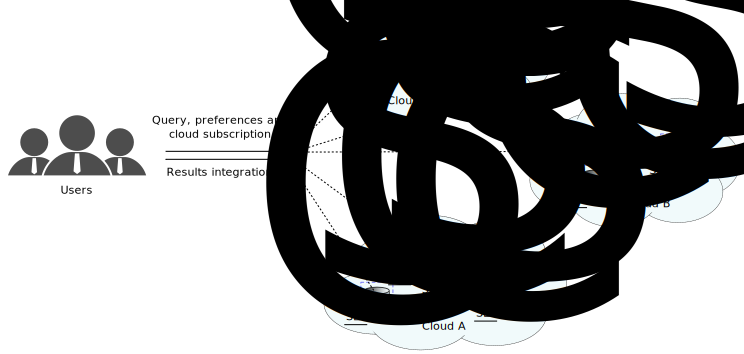
\includegraphics[scale=0.40]{scenario.pdf}
\caption{Data integration scenario}\label{fig:scenario}
\end{figure}

In our work, we consider a new vision of data integration in a multi-cloud context (see figure~\ref{fig:scenario}). Data is accessed and retrieved as \textit{data services} deployed in \textit{cloud providers} geographically distributed. \textit{Data services} and \textit{cloud providers} export their SLA specifying the level of services they can guarantee to users. Two types of SLA are considered: (1) cloud SLA (SLA$_{C}$), agreements between a \textit{data service} and a \textit{cloud provider}; and (2) service SLA (SLA$_{S}$), agreements between \textit{users} and \textit{data services}. The figure~\ref{fig:cloudsla} illustrates a cloud SLA schema.  

\begin{figure*}[th!]
\center
\includegraphics[scale=0.57]{Cloud_SLA.pdf}
\caption{Cloud SLA}\label{fig:cloudsla}
\end{figure*}

Therefore, given a user query, her integration quality requirements and her cloud subscription, it is rewritten in terms of cloud services (\textit{data services} and \textit{data processing services}) composition that fulfill the integration requirements and deliver the expected results to the user. This new vision brings challenges to data integration, such as:
\begin{itemize}
\item \textbf{Performance}. In the multi-cloud, we are dealing with a huge amount of \textit{data services}, \textit{data processing services} and \textit{cloud providers}. Consequently, producing and executing service compositions can require an important quantity of resources and processing time.
\item \textbf{Economic model}. Even with the possibility of having an unlimited access to resources, the user is limited to the resources she has contracted and to the budget she is ready to pay for. Thus, it is crucial to design new methods in order to produce rewritings which satisfies the user integration requirements and the cloud economic model. 
\item \textbf{Quality issues}. Some rewritings produced and executed to the user query could not satisfy her quality requirements concerning privacy, data provenance, cost, among others. Producing and executing these rewritings implies increasing time processing and integration total cost. 
\item \textbf{SLA heterogeneity}. While producing the rewritings, it is necessary to match the user requirements with the different SLAs exported by the \textit{cloud providers} and \textit{cloud services}. In the multi-cloud, \textit{cloud providers} and \textit{cloud services} export SLAs with different semantics and structure that makes the matching SLA and user requirement challenging. In addition, we are also dealing with incompatibilities of SLAs.
\item \textbf{Reuse}. Rewriting and executing the user query is computationally costly in terms of processing time and economic cost. Thus, it is necessary to propose a manner of reusing previous integration in order to save time and money, but also meeting the user expectations.
\end{itemize}

\subsection{SLA-based data integration approach}
Motivated by the challenges discussed in the previous section, we propose our SLA-based data integration approach to multi-cloud environments. The data integration process includes (i) looking up services that can be used as \textit{data services}, and for services required to process the retrieved data and build an integrated result (called \textit{data processing services}); (ii) processing data retrieval, processing and integration; and (iii) delivering results to the user considering her quality requirements, context and resource consumption.  In this sense, our approach is divided in four steps. Given a user \textit{query}, a set of user \textit{preferences} associated to it, \textit{cloud providers} and \textit{cloud services}:
\\
\textbf{\underline{SLA derivation}}. In this step, we compute what we call an \textsl{integrated
SLA} that matches (including quality constraints and data requirements) with the SLA's provided by \textit{cloud services}, given a specific user cloud subscription. The user may have general \textit{preferences} depending on the context she wants to integrate her data such as economic cost, bandwidth limit, free services, and storage and processing limits. The \textit{SLA derivation} is the big challenge while dealing with SLAs and particularly for adding quality dimensions to data integration. Furthermore, the \textsl{integrated SLA} guides the query evaluation, and the way results are computed and delivered. \\
\textbf{\underline{Filtering data services}}. The \textsl{integrated SLA} is used (i)
to filter previous SLA derived for a similar request in order to reuse previous results; or (ii) to filter possible \textit{cloud services} that can be used for answering the query. The SLA exported by a selected \textit{cloud service} should satisfy the user \textit{preferences}. \\
\textbf{\underline{Query rewriting}}. Given a set of \textit{data services} that can
potentially provide data for integrating the query result, a set of service compositions is generated according to the \textsl{integrated SLA} and the agreed SLA of each \textit{data services}. \\
\textbf{\underline{Integrating a query result}}. The service compositions are executed
in one or several clouds where the user has a subscription. The execution cost of service compositions must fulfill the \textsl{integrated SLA}. The clouds resources needed to execute the composition and how to use them is decided taking in consideration the economic cost determined by the data to be transferred, the number of external calls to services, data storage and delivery cost.

%\subsection{SLA model}

\subsection{Query rewriting algorithm}
To serve as a proof of concept to our approach, we intend to develop a query
rewriting algorithm which is guided by users' integration requirements and
service level agreements exported by different data services and cloud
providers. The query rewriting is an important issue in data integration. In
cloud computing, researches have refereed to it as a service composition problem
in which given a query the objective is to lookup and compose data services that
can contribute to produce a result. \cite{Barhamgi2010} proposed a query
rewriting approach which processes queries on data provider services.
\cite{Benouaret2011} introduced a service composition framework to answer
preference queries. Two algorithms inspired on~\cite{Barhamgi2010} are presented
to rank the best rewritings based on previously computed scores. \cite{ba2014}
extended \cite{Umberto} and presented an refinement algorithm that produces and
order rewritings according to user preferences and scores. In general, these
works share the same performance problem depending on the size of the query and
on the number of available services. Furthermore, they do not take into
consideration user's integration requirements what can lead to produce
rewritings that are not satisfactory to the user in terms of quality
requirements and cost. Currently, we have formalized and developed a rewriting
algorithm that considers user preferences and services' quality aspects while
selecting services and producing rewritings.                    

PREPARAR UMA ESTRUTURA GERAL PARA O AGORITMO MULTI CLOUD
\begin{algorithm} 
%\small
\caption{ - \ldots}
\label{qualityBasedAlgorithm}
\begin{algorithmic}[1]
\REQUIRE Query ($Q$), user preferences ($P$), user cloud subscription ($C$) and a set of previous \textit{integrated SLA} ($\bigSLA$).
\ENSURE Integration results delivered considering the user context (cloud subscription).
%\STATE \textbf{function} $\mathit{SelectCandidateServices} (Q, \bigS)$
%\STATE let $\bigSLA$ be a set of previous integrated SLA
\STATE $pI \leftarrow \emptyset$
\FORALL  {$SLA_{i}$ in $\bigSLA$}
	\IF {$\mathit{macthes(Q, P, SLA_{i})}$}
		\STATE $pI \leftarrow pI \cup \lbrace SLA_{i} \rbrace$		
%		\FORALL  {$A_{j}$ in $S_{i}$}
%			\IF {$Q.\mathit{notContains(A_{i})}$}
%				\STATE $b \leftarrow \mathit{false}$	
%				\STATE $\mathit{break}$
%			\ENDIF
%		\ENDFOR
%		\IF {$b = true$}
%			\STATE $\bigLS \leftarrow \bigLS \cup \lbrace S_{i} \rbrace$	
%		\ENDIF
	\ENDIF
\ENDFOR
\IF {$pI \neq \emptyset$}
	\STATE $sI \leftarrow chooseBest(P, pI)$
	\STATE $newSLA_{i} \leftarrow deriveSLA(sI, P, C)$
%	\FORALL  {$SLA_{i}$ in $pI$}
%		\STATE $sI \leftarrow choose(P,)$
%	\ENDFOR
\ELSE
	\STATE $newSLA_{i} \leftarrow deriveSLA(Q, P, C)$
	\STATE $newSLA_{i} \leftarrow updateSLA(Rhone(newSLA_{i}))$
\ENDIF
\STATE $IR \leftarrow execute(newSLA_{i})$
\STATE \textbf{return} $IR$
\STATE \textbf{end function}
\end{algorithmic}
\end{algorithm} 

\section{Preliminary results}
We have developed a prototype of our query rewriting algorithm (called \textit{Rhone}) which takes into consideration users' requirements and services' quality aspects extracted from SLAs.
The Rhone prototype is implemented in Java.
It includes 15 java classes in which 14 of them model the basic concepts 
(\textit{query}, \textit{abstract services}, \textit{concrete services}, etc), 
and 1 responsible to implement the core of the algorithm. 

Currently, our approach runs in a controlled environment. 
Different experiments were produced to analyze the algorithm's behavior.
We will present two experiments: \textit{experiment 1} and \textit{experiment 2}.
The service registry used has 100 concrete services. 
In each experiment, there are a set of tests in which the number of concrete 
services varies from 5 until to reach 100.

\begin{figure}[!h]
\centering
\includegraphics[scale=0.8]{fig1.pdf}
\caption{Performance evaluation.}\label{fig01}
\end{figure} 

The \textit{experiment 2} (figure~\ref{fig:fig02}) presents the results while testing the algorithm in the presence of user preferences and services' quality aspects extracted from SLAs.  The difference between \textit{Test 1} and \textit{Test 2} concerns the way services are selected and the query is rewritten. Once \textit{Test 1} do not consider quality measures as any other existing query rewriting approach, \textit{Test 2} uses the user preferences statements and services' quality aspects to guide the service selection and query rewriting.
Both include queries with six abstract services and quality requirements concerning availability, response time, price per call and integration cost (total cost). The figure~\ref{fig:fig02} shows our results. 

%\begin{figure}%
%\centering
%\parbox{2.2in}{\includegraphics[scale=0.30]{exp2.png}}% 
%\qquad
%\begin{minipage}{2in}%
%\includegraphics[scale=0.30]{exp3.png}
%\end{minipage}%
%\caption{Results concerning processing time (left-side) and rewritings number (right-side).}%
%\label{fig:fig02}%
%\end{figure}

\begin{figure}[!h]
\centering
\includegraphics[scale=0.8]{fig2.pdf}
\caption{Performance evaluation.}\label{fig02}
\end{figure} 

The results while considering user preferences and SLAs are promisingly.  
%The \textit{Rhone} presents a better performance, decreasing the processing time and 
%the total number of rewritings produced.  
%Reducing rewriting number allow to go straightforward to the rewriting solutions that are satisfactory avoiding any further backtrack.
The \textit{Rhone} increases performance reducing rewriting number (around 50 percent) which allows to go straightforward to the rewriting solutions that are satisfactory avoiding any further backtrack and thus reducing successful integration time. Moreover, once the services selection and service composition (rewritings) process are fully guided by the user requirements and SLA, the algorithm avoid producing and executing composition that are not interest for the user. In this sense, the reduces the integration economic cost while delivering the expected results.

\section{Conclusions and Research plan}
This paper introduces a new vision of data integration adapted to the cloud economic model. It also proposes a new approach for data integration based on user integration requirements and SLA. In addition, an query rewriting algorithm called \textit{Rhone} servers as proof of concept. Our preliminary results have shown that the \textit{Rhone} reduces the rewriting number and processing time while considering user preferences and services' quality aspects extracted from SLAs to guide the service selection and rewriting. Furthermore, the integration quality is enhanced, and it is adapted to cloud economic model reducing the total cost of the integration.

 
\bibliographystyle{splncs03} 
\bibliography{bibliography}

\end{document}